% - The xcolor package with the x11names options defines several colors,
%   e.g. DeepSkyBlue4 which is used in template/beamer-template-original.tex
% - compress: Tries to make all navigation bars as small as possible
% - fleqn: Position equations at a fixed indent from the left margin 
%   rather than centered in the text column
\documentclass[10pt,xcolor=x11names,compress,fleqn]{beamer}

% If you're happy with the look of this presentation showcase, you can
% copy the following two lines to your tex document. You then have to
% copy the libs and template folder to your presentation folder as well.
% If you want to use different packages or change certain commands, you 
% might want to place your changes inside the libs folder!
\usepackage[english]{babel}

% Used in template/beamer-template-extended-same-slide-number-for-allow-frame-breaks.tex
\usepackage{xpatch}
% Used in contents/example-math.tex
\usepackage{amsmath}
% Used in contents/example-tikz.tex
\usepackage{tikz}
% Example use of this command can be found in contents/example-tables.tex (first example)
% Needed to create below command.
\usepackage{array}
\newcolumntype{C}[1]{>{\centering\let\newline\\\arraybackslash\hspace{0pt}}m{#1}}

% Example use of this command can be found in contents/example-tables.tex (first example, second example)
% Provides \toprule, \midrule, \bottomrule
\usepackage{booktabs}

% Example use of this command can be found in contents/example-tables.tex (second example)
% Provides \multirow
\usepackage{multirow}

% Taken from https://tex.stackexchange.com/a/45038/30325
% Example: content/example-separating-slide.tex
\makeatletter
\let\beamer@writeslidentry@miniframeson=\beamer@writeslidentry
\def\beamer@writeslidentry@miniframesoff{%
  \expandafter\beamer@ifempty\expandafter{\beamer@framestartpage}{}% does not happen normally
  {%else
    % removed \addtocontents commands
    \clearpage\beamer@notesactions%
  }
}
\newcommand*{\miniframeson}{\let\beamer@writeslidentry=\beamer@writeslidentry@miniframeson}
\newcommand*{\miniframesoff}{\let\beamer@writeslidentry=\beamer@writeslidentry@miniframesoff}
\makeatother
% Taken from http://tex.stackexchange.com/a/33973/30325:
% Smaller font for references.
% Example use of this command can be found in contents/example-sources-listed-in-appendix.tex
\newcommand\Fontvi{\fontsize{6}{7.2}\selectfont}
% Taken from https://web.archive.org/web/20091217203809/http://cameron.bracken.bz/beamer-template

%%%%%%%%%%%%%%%%%%%%%%%%%%%%%%%%%%%%%%%%%%%%%%%%%%%%%%%%%%%%
%%  This Beamer template was created by Cameron Bracken.
%%  Anyone can freely use or modify it for any purpose
%%  without attribution.
%%
%%  Last Modified: January 9, 2009
%%

\useoutertheme[subsection=false,shadow]{miniframes}
\useinnertheme{default}
\usefonttheme{serif}
\usepackage{palatino}

\setbeamerfont{title like}{shape=\scshape}
\setbeamerfont{frametitle}{shape=\scshape}

\setbeamercolor*{lower separation line head}{bg=DeepSkyBlue4} 
\setbeamercolor*{normal text}{fg=black,bg=white} 
\setbeamercolor*{alerted text}{fg=red} 
\setbeamercolor*{example text}{fg=black} 
\setbeamercolor*{structure}{fg=black} 
 
\setbeamercolor*{palette tertiary}{fg=black,bg=black!10} 
\setbeamercolor*{palette quaternary}{fg=black,bg=black!10} 
% Taken from https://tex.stackexchange.com/questions/370485/increasing-space-between-title-and-date-beamer-class
\makeatletter
\setbeamertemplate{title page}{%
  \vbox{}
% \vfill
% \vspace{3.5cm}% NEW
  \begingroup
    \centering
    \begin{beamercolorbox}[sep=8pt,center]{title}
      \usebeamerfont{title}\inserttitle\par%
      \ifx\insertsubtitle\@empty%
      \else%
        \vskip0.25em%
        {\usebeamerfont{subtitle}\usebeamercolor[fg]{subtitle}\insertsubtitle\par}%
      \fi%     
    \end{beamercolorbox}%
    \vskip1em\par
    \begin{beamercolorbox}[sep=8pt,center]{author}
      \usebeamerfont{author}\insertauthor
    \end{beamercolorbox}
    \begin{beamercolorbox}[sep=8pt,center]{institute}
      \usebeamerfont{institute}\insertinstitute
    \end{beamercolorbox}
%   \vspace{1.5cm}% NEW
    \begin{beamercolorbox}[sep=8pt,center]{date}
      \usebeamerfont{date}\insertdate
    \end{beamercolorbox}\vskip0.5em
%    {\usebeamercolor[fg]{titlegraphic}\inserttitlegraphic\par}
  \endgroup
% \vfill
}
\makeatother
% Use circle for non numbered items in listings. 
% Example use of this command can be found in contents/example-listing-normal.tex
\setbeamertemplate{itemize items}[circle]

% This makes text which is hidden by the \pause command 
% (see contents/example-uncover-slide-piecewise.tex) not 
% appear invisible, but gray
\setbeamercovered{transparent}
% Taken from https://tex.stackexchange.com/a/688
% Get rid of default navigation symbols.
% Used in all slides.
\setbeamertemplate{navigation symbols}{} 

% Show frame numbers.
% Used in all slides.
\setbeamertemplate{footline}[frame number]  

% Show frame numbers in gray color.
% Used in all slides.
\setbeamercolor{page number in head/foot}{fg=gray}
% Taken from https://tex.stackexchange.com/a/124271
% Show numbers instead of icons.

% Example use of this command can be found in contents/example-sources-listed-in-appendix.tex

\setbeamertemplate{bibliography item}{[\theenumiv]}
% Taken from https://golatex.de/viewtopic.php?f=5&t=23907
% According to https://golatex.de/viewtopic.php?f=22&t=23909&p=116101#p116101 the following code 
% therefore is licensed under Attribution-ShareAlike 4.0 International (CC BY-SA 4.0). The author
% is the member Grummelgast of the golatex forum. The content of the aforementoined license can be
% found in the LICENSE.md file at the root level of this repository.
% Example use of this command can be found in contents/example-sources-listed-in-appendix.tex
\newcounter{multipleslide}
\newif\ifmultipleslide
\xapptocmd{\multipleslidetrue}{\setcounter{multipleslide}{\value{framenumber}}\stepcounter{multipleslide}}{}{\PatchFailure}
\xapptocmd{\multipleslidefalse}{\setcounter{framenumber}{\value{multipleslide}}}{}{\PatchFailure}
\xpretocmd{\insertframenumber}{\ifmultipleslide \themultipleslide\else}{}{\PatchFailure}
\apptocmd{\insertframenumber}{\fi}{}{\PatchFailure}

% You can modify this file to change what's being displayed on the title slide
\title{Title of presentation}
\subtitle{Subtitle of presentation}
\institute{Name of event\\Name of organisation}
\author{Name of lecturer}
\date{\today}

\begin{document}

  % Don't modify these two slides if you're happy with the look of this
  % presentation showcase
  \begin{frame}[plain]

  \titlepage

\end{frame}
  \begin{frame}
  
  \frametitle{Table of contents}
  \tableofcontents[hideallsubsections]

\end{frame}
  
  % -----------------------------------------------------------------------------
  % Here start part which defines which content is displayed in the presentation!
  % (except for the title slide, see line 16)
  % -----------------------------------------------------------------------------
  \section{\scshape Sections}  
  % This makes the slide not appear in the navigation bar as a dot
\miniframesoff

\begin{frame}{}

  \centering
  {\LARGE\textsc{Sections\\\vspace{0.2cm}\tiny{(This is a separating, kind of blank slide to introduce a new section)}}}
  
\end{frame}
  
\miniframeson
  \subsection{First subsection}

\begin{frame}{Sections and subsections}

  For each \textit{\textbackslash section\{title\}} you put into your latex document, \textit{title} will appear in the \textit{table of contents} slide and in the navigation bar at the top. \\
  
  \vspace{0.4cm}
  
  For each slide which comes after a \textit{\textbackslash section\{title\}}, a dot will appear in the navigation bar below the corresponding \textit{title}. The dot will be filled if you visit the according slide. However, you can turn  off that a dot will be shown for individual slides if you use \textit{\textbackslash miniframesoff/on}. For example, go to the previous slide - no highlighted dot is shown for this slide!
    
  \vspace{0.4cm}
  
  You can group slides into subsections, too, by using \textit{\textbackslash subsection\{title\}}. This has the effect that the dots at the navigation bars are grouped together. Too see this effect, please take a look at the dots while visiting the following slides!
  
\end{frame}

\subsection{Second subsection}

\begin{frame}{}

  First slide of second subsection.

\end{frame}

\begin{frame}{}

  Second slide of second subsection.

\end{frame}

\subsection{Third subsection}

\begin{frame}{}

  First slide of third subsection.

\end{frame}

\begin{frame}{}

  Second slide of third subsection.

\end{frame}
  
  \section{\scshape Listings}  
  \begin{frame}{Normal listing example}

  An \textit{itemize} listing:

  \begin{itemize}
    \item First item
    \item Second item
  \end{itemize}

  \vspace{0.6cm}

  An \textit{enumerate} listing:

  \begin{enumerate}
    \item First item
    \item Second item
  \end{enumerate}

  \vspace{0.6cm}

  An \textit{enumerate} listing with different symbols:

  \begin{enumerate}[1)]
    \item First item
    \item Second item
  \end{enumerate}

\end{frame}

\begin{frame}{Nested listing example}

  \begin{itemize}

    \item First main item:

    \begin{itemize}
      \item First item
      \item Second item
    \end{itemize}
    
    \vspace{0.6cm}

    \item Second main item:

    \begin{itemize}
      \item First item
      \item Second item
    \end{itemize}

  \end{itemize}

\end{frame}
  
  \section{\scshape Tables}
  \begin{frame}{Table example \#1}

  \begin{table}[htb]

    \centering
  
    % Instead of using the special C{Xcm} command you could use a regular "c" instead for having centered columns (try it!), 
    % but then the columns would be too wide. Giving a specific cm width prevents this.
    \begin{tabular}{ C{1.5cm}      C{0.9cm}       C{2.0cm}                  C{1.5cm}                C{2.3cm}}
                                 & \# targ. ads & Sites only Prec./Recall & Ads only Prec./Recall & Ads \& Sites Prec./Recall \\
       \toprule
                     Same cat.   & 22           & 20/10                   & 16/8                  & 17/18 \\
       \hline                       
                     Same parent & 17           & 54/34                   & 51/24                 & 53/50\\
       \hline                       
                     Same root   & 14           & 76/61                   & 82/40                 & 79/81\\
       \bottomrule
       
    \end{tabular}

    \caption{Almost a standard table (except for the fixed with of the columns)}

  \end{table}

\end{frame}

\begin{frame}{Table example \#2}

  \begin{table}[htb]
  
    \centering

    \begin{tabular}{lll}
      \toprule  
      Vertraulichkeit & Integrität &  Integritätsprüfung \\
      \midrule    

      \multirow{4.4}{*}{\shortstack[l]{AES/CTR\\(SPOC)\\(eSPOC)\\(PCoding)}} & 
      \multirow{2}{*}{HMAC} & 
      \multirow{2}{*}{E} \\

      & & \\ 
      \cmidrule(rl){2-3}

      & \multirow{2}{*}{ECDSA} & \multirow{2}{*}{E, (Z+E)} \\

      &  & \\
      \bottomrule
    \end{tabular}

    \caption{A special table in which one vertical line doesn't span all columns}

  \end{table}
  
\end{frame}
  
  \section{\scshape Images}
  \begin{frame}{Image example}

  \vspace{0.3cm}

  \begin{figure}
    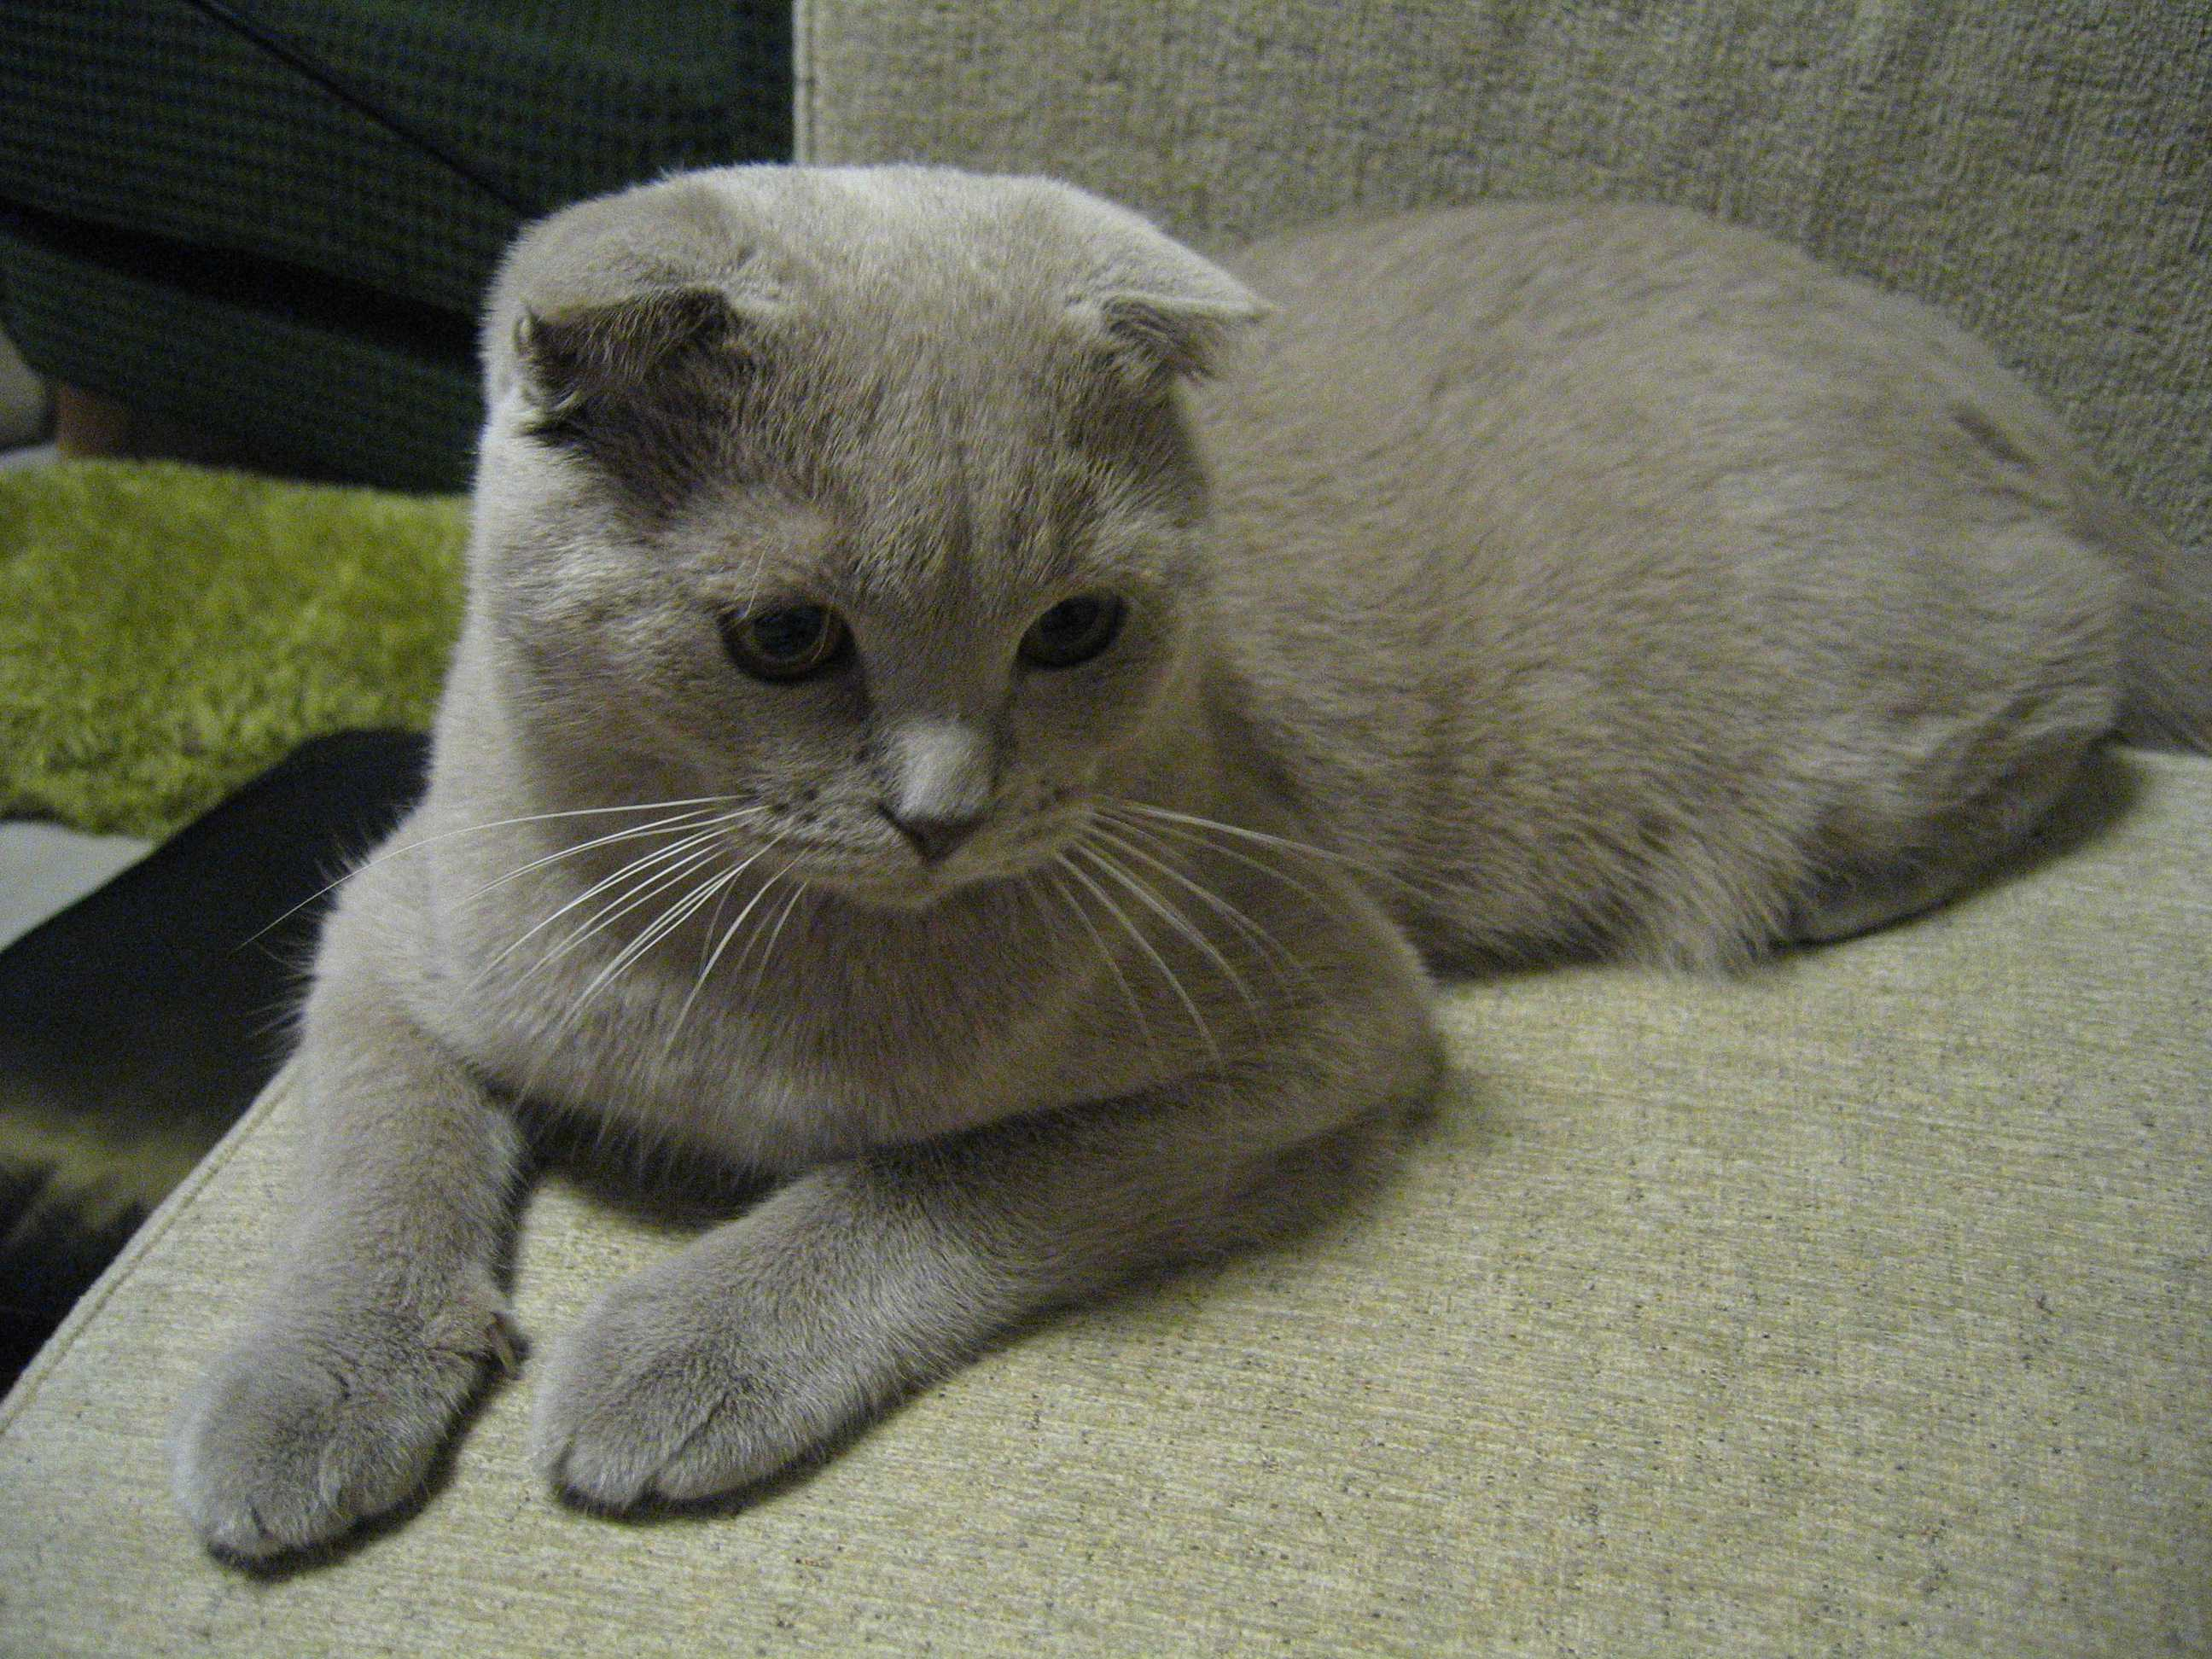
\includegraphics[width=0.6\textwidth]{images/cat-1.jpg}
    \caption{A picture of a cat!}
  \end{figure}
  
  The image above is in pulibc domain. Therefore it's not mandatory to give credit. 

\end{frame}
  
  \section{\scshape Citing sources}
  \begin{frame}{Sources cited in slide example}

  This is a sentence which cites a source. \cite{Ahlswede2000-1} \\
  Click on the source citation to go to the source chapter.

  \vspace{0.3cm}

  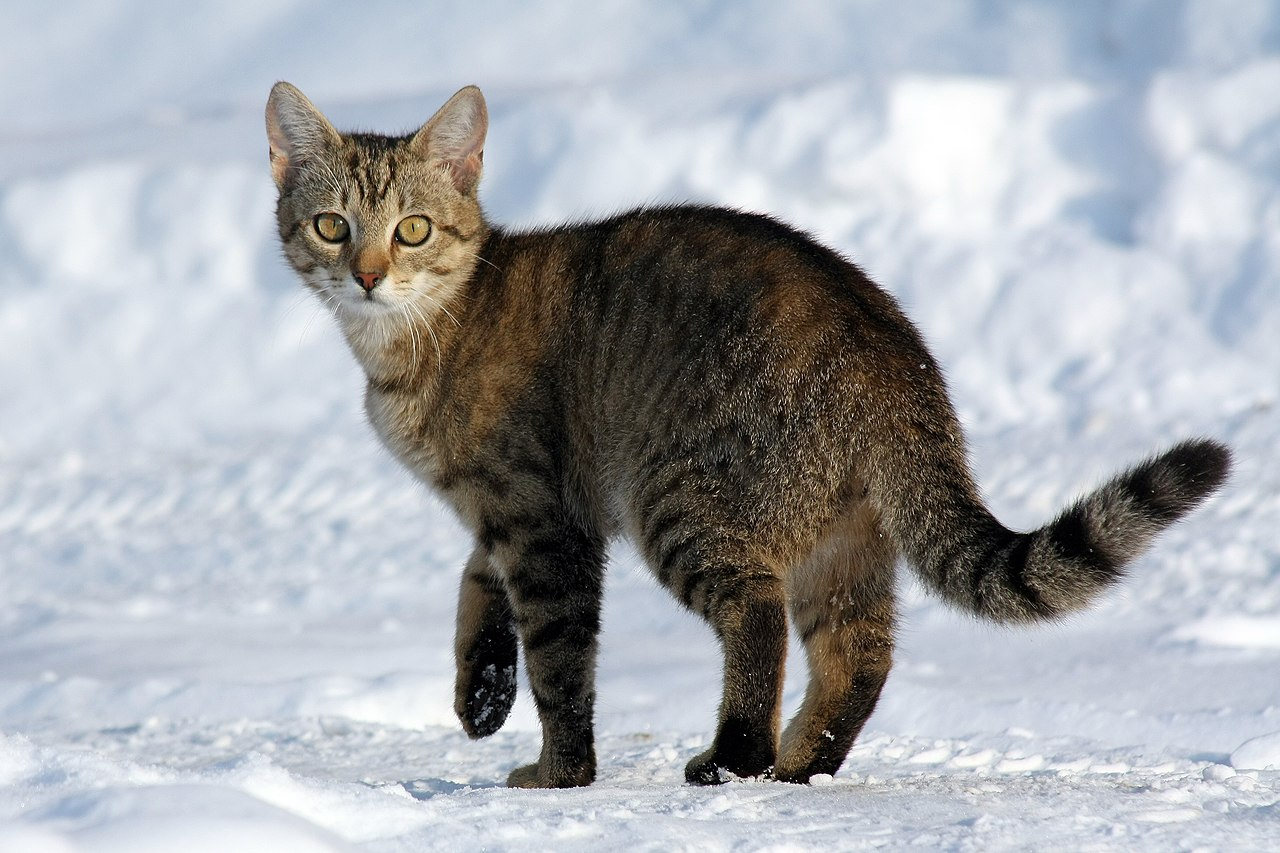
\includegraphics[width=0.6\textwidth]{images/cat-2.jpg}
  
  \vspace{0.3cm}
  
  You can also put source citations at the bottom left of the page. \\
  Here we use this for the picture above.

  \citeAtFooter{\cite{cat-2}}
		
\end{frame}

  
  \section{\scshape Other}
  
  \subsection{Blocks}
  \begin{frame}{Block example}

  A \textit{block} is a block of text which has a heading:

  \begin{block}{Theorem}
    The description of the theorem goes here.
  \end{block}

\end{frame}
  
  \subsection{Math}
  \subsection{Math}
  
\begin{frame}{Math example}

  It's possible to display math equations in latex presentations, too:

  \begin{align*}
   f(x) &= (x+a)(x+b) \\
        &= x^2 + (a+b)x + ab
  \end{align*}

\end{frame}
  
  \subsection{TikZ}
  \subsection{TikZ}

\begin{frame}{Tikz example}

  The Tikz library can be used to create diagrams:
  
  \vspace{0.4cm}

  \begin{figure}
    \centering
    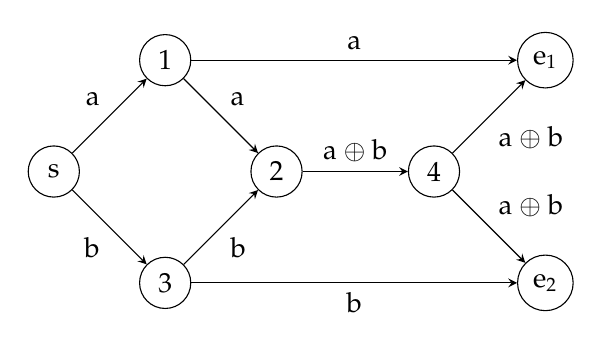
\begin{tikzpicture}[->,>=stealth,node distance=2cm,
	main/.style={shape=circle, draw=black, minimum size=6.5mm},
	empty/.style={}];
	\node[main] (1) [] {s};
	\node[main] (2) [above right of=1] {1};
	\node[main] (3) [below right of=2] {2};
	\node[main] (4) [below right of=1] {3};
	
	\node[main] (5) [right of=3,] {4};
	\node[main] (6) [above right of=5] {e\textsubscript{1}};
	\node[main] (7) [below right of=5] {e\textsubscript{2}};
	
	\path
	(1) edge node [above left] {a} (2)
	(1) edge node [below left] {b} (4)
	(2) edge node [above right] {a} (3)
	(4) edge node [below right] {b} (3)
	(3) edge node [above] {a $\oplus$ b} (5)
	(5) edge node [below right] {a $\oplus$ b} (6)
	(5) edge node [above right] {a $\oplus$ b} (7)
	(2) edge node [above] {a} (6)
	(4) edge node [below] {b} (7);
\end{tikzpicture}
    \caption{A diagram created with Tikz}
  \end{figure}

\end{frame}
  
  \subsection{Alignment}
  \subsection{Alignment}
  
\begin{frame}{Alignment example}

  The equations below are aligned side by side:
  
  \begin{columns}
    \column{.5\textwidth}
    \begin{align*}
        &y^2 \stackrel{\times}{=}{(\lceil \sqrt[]{n} \rceil)}^2 \hphantom{+1)} -n \\ 
        &y^2 \stackrel{\times}{=}{(\lceil \sqrt[]{n} \rceil+1)}^2 -n \\
        &... \\
        &y^2  \stackrel{\checkmark}{=}{(\lceil \sqrt[]{n} \rceil+z)}^2 -n \\ 
    \end{align*}
    \column{.5\textwidth}
    \begin{align*}
        & n = 119,\sqrt[]{n}=10.9 \\
        & y^2 \stackrel{\times}{=}{11}^2 -119 = 30  \\
        & y^2 \stackrel{\checkmark}{=}{12}^2 -119 = 25  \\
        & \hphantom{y^2}\rightarrow x=12, y = 5 \\
        & n=(12+5) \cdot (12-5) \\
    \end{align*}
  \end{columns}

\end{frame}
  
  \subsection{Slide numbers}   
  \begin{frame}{Slide numbers}

  Take a look at the slide numbers at the bottom right! 

  \begin{itemize}
    \item At the title slide no slide number is given
    \item The \textit{Sources} at the end of the presentation
          comprise multiple slides. Nevertheless, the slide 
          numbers don't increase by more than one. This is due
          to using the \textit{multipleslidetrue/false} command
          in combination with the \textit{allowframebreaks}
          option.
  \end{itemize}

\end{frame}
  
  \subsection{Uncover a slide piecewise}
  \begin{frame}{Uncover a slide piecewise example}

  \begin{itemize}
    \item A slide can be uncovered piece by piece! \pause
    \item First item 
    \item Second item \pause
  \end{itemize}
  
  \vspace{0.4cm}
  
  Notice that the slide numbers didn't change while uncovering the slide! The same is true for the filled dot at the navigation bar at the top!

\end{frame}
  
  \section{\scshape Sources}   
  \multipleslidetrue
\begin{frame}[allowframebreaks]{Sources}   

  % Regarding the second argument of "thebibliography": 
  % "If you use numeric labels, then the argument should be a single digit (9 is commonly used),
  % if there are less than ten items; two digits (commonly 99) if there are from 10 to 99 items and so on."
  % https://tex.stackexchange.com/questions/198330/argument-in-thebibliography 
  \begin{thebibliography}{9}  

    \Fontvi

    \bibitem{Ahlswede2000-1}
    \textsc{Ahlswede}, R ; \textsc{Cai}, Ning  ; \textsc{Li},
      S.Y. ; \textsc{Yeung},  R.W:
    \newblock Network Information Flow
    \newblock {In: }\emph{IEEE Transactions on Information Theory 46 (2000), September, Nr. 4, 1204-1216}
    \newblock http://dx.doi.org/10.1109/18.850663
    \newblock DOI 10.1109/18.850663
    \newblock ISSN 0018–9448

    \bibitem{Ahlswede2000-2}
    \textsc{Ahlswede}, R ; \textsc{Cai}, Ning  ; \textsc{Li},
      S.Y. ; \textsc{Yeung},  R.W:
    \newblock Network Information Flow
    \newblock {In: }\emph{IEEE Transactions on Information Theory 46 (2000), September, Nr. 4, 1204-1216}
    \newblock http://dx.doi.org/10.1109/18.850663
    \newblock DOI 10.1109/18.850663
    \newblock ISSN 0018–9448

    \bibitem{Ahlswede2000-3}
    \textsc{Ahlswede}, R ; \textsc{Cai}, Ning  ; \textsc{Li},
      S.Y. ; \textsc{Yeung},  R.W:
    \newblock Network Information Flow
    \newblock {In: }\emph{IEEE Transactions on Information Theory 46 (2000), September, Nr. 4, 1204-1216}
    \newblock http://dx.doi.org/10.1109/18.850663
    \newblock DOI 10.1109/18.850663
    \newblock ISSN 0018–9448

    \bibitem{Ahlswede2000-4}
    \textsc{Ahlswede}, R ; \textsc{Cai}, Ning  ; \textsc{Li},
      S.Y. ; \textsc{Yeung},  R.W:
    \newblock Network Information Flow
    \newblock {In: }\emph{IEEE Transactions on Information Theory 46 (2000), September, Nr. 4, 1204-1216}
    \newblock http://dx.doi.org/10.1109/18.850663
    \newblock DOI 10.1109/18.850663
    \newblock ISSN 0018–9448

    \bibitem{Ahlswede2000-5}
    \textsc{Ahlswede}, R ; \textsc{Cai}, Ning  ; \textsc{Li},
      S.Y. ; \textsc{Yeung},  R.W:
    \newblock Network Information Flow
    \newblock {In: }\emph{IEEE Transactions on Information Theory 46 (2000), September, Nr. 4, 1204-1216}
    \newblock http://dx.doi.org/10.1109/18.850663
    \newblock DOI 10.1109/18.850663
    \newblock ISSN 0018–9448

    \bibitem{Ahlswede2000-6}
    \textsc{Ahlswede}, R ; \textsc{Cai}, Ning  ; \textsc{Li},
      S.Y. ; \textsc{Yeung},  R.W:
    \newblock Network Information Flow
    \newblock {In: }\emph{IEEE Transactions on Information Theory 46 (2000), September, Nr. 4, 1204-1216}
    \newblock http://dx.doi.org/10.1109/18.850663
    \newblock DOI 10.1109/18.850663
    \newblock ISSN 0018–9448

    \bibitem{Ahlswede2000-7}
    \textsc{Ahlswede}, R ; \textsc{Cai}, Ning  ; \textsc{Li},
      S.Y. ; \textsc{Yeung},  R.W:
    \newblock Network Information Flow
    \newblock {In: }\emph{IEEE Transactions on Information Theory 46 (2000), September, Nr. 4, 1204-1216}
    \newblock http://dx.doi.org/10.1109/18.850663
    \newblock DOI 10.1109/18.850663
    \newblock ISSN 0018–9448

    \bibitem{Ahlswede2000-8}
    \textsc{Ahlswede}, R ; \textsc{Cai}, Ning  ; \textsc{Li},
      S.Y. ; \textsc{Yeung},  R.W:
    \newblock Network Information Flow
    \newblock {In: }\emph{IEEE Transactions on Information Theory 46 (2000), September, Nr. 4, 1204-1216}
    \newblock http://dx.doi.org/10.1109/18.850663
    \newblock DOI 10.1109/18.850663
    \newblock ISSN 0018–9448

  \end{thebibliography} 
  
\end{frame}
\multipleslidefalse
		
\end{document}